\documentclass[16.7pt]{jsarticle}

\usepackage{SPR}

\headerSPR
\begin{document}
	\titleSPR{\number\year}{\number\month}{\number\day}{D2}{吉田 皓太郎}
%%%%%%%%%%%%%%%%%%%%%%%%%%%%%%%%%%%%%%
	%\articleSPRabst
	%	\begin{itemize}
	%		\item =どういう事態か
	%	\end{itemize}
		
%今回のMTGの目的,何をディスカッションし,結果に何を得たいのかを決定する.※ミーティングごとに記入
	\articleSPRobj
		今回のMTGでは,D論の構成を現状までに達成された項目に基づき考察・再構築したものを記載しており,先生の意見を踏まえD論構成を確定させたいと考えている.また,そのD論構成に基づいた時,残りの少ない時間で何を行うべきかを議論し,今後の計画へと繋げたいと考えている.
		

%%%%%%%%%%%%%%%%%%%%%%%%%%%%%%%%%%%%%%
% 1.前回からのノルマ
	\articleSPRitemsone
		%\begin{enumerate}
		%	\item A
		%\end{enumerate}
		
		\tableofcontents
		
		
%%%%%%%%%%%%%%%%%%%%%%%%%%%%%%%%%%%%%%
%\begin{itemize}
%	\item 新規手法について
%	\item ISFAアウトライン
%\end{itemize}
%%%%%%%%%%%%%%%%%%%%%%%%%%%%%%%%%%%%%%
% 2.具体的な成果
	\articleSPRitemstwo
	\renewcommand{\labelitemi}{$\blacktriangledown$}
	%\renewcommand{\labelitemi}{$\bigcirc$}
	\newcommand{\argmax}{\mathop{\rm arg~max}\limits}
	\newcommand{\argmin}{\mathop{\rm arg~min}\limits}
	\newcommand{\Ker}{{\rm Ker}}
	\newcommand{\rank}{{\rm rank}}
%%%%%%%%%%%%%%%%%%%%%%%%%%%%%%%%%%%%%
	\section{局所修正法について}
		前回のMTGではそもそも計算の定義が間違っており,実行できませんでした.
		
		この修正作業については,今までとそこまで解法の変わり映えしないという理由もあり,アルゴリズムによって修正作業を達成することを考えます.
		
		\subsection{アルゴリズムの考え方と諸定理について}
			本研究の着想の根本は,目標点に対してSCIで発表したように一度に移動させるのではなく,繰り返し修正操作を繰り返すことによって,点を満たすように移動することを考えたいと思います.
		
			それを踏まえて,一度今までの式を振り返ります.
			ある$ \varepsilon_c $および$ \bd{d} $に対して,修正後の長さ分布$ \varepsilon(s) $は,$ \bd{d} $が$ s $によって変化しない仮定の下で次式で表されます.
			\begin{equation}\label{eq:varDiffeq}
				\varepsilon' = -\frac{|u'\zetav_U\times \zetav_L|}{D \cos \alpha} \mathrm{sgn}((\zetav_L \times \zetav_U) \cdot \etav)\varepsilon := \sigma \varepsilon
			\end{equation}
			
			この式が$ s = s_c $で$ \varepsilon=\varepsilon_c $を取るならば,一意に
			\begin{equation}\label{eq:vareq}
				\varepsilon = \varepsilon_c \exp \left[ \int_{s_c}^{s} \sigma ds \right]
			\end{equation}
			と表されます.
			
			次に,母線の分布に沿って曲線を操作するときには,どのような$ \varepsilon $の分布を選んでも,可展面の式を満たすことができることを証明する.変更方向が母線分布に合わせて変化するとき,可展面の接平面式を求めると,
			\begin{equation}\label{eq:TanEq_withGene}
				\left\{ (u'\zetav_U + \varepsilon' \bd{d}_2 + \varepsilon \bd{d}_2') \times \zetav_L \right\}\cdot(D+\varepsilon)\bd{d}_2 = 0
			\end{equation}
			となります.計算過程では,$ \xv_U - \xv_L = D \bd{d}_2 $であることを用いている.スカラー3重積の変換操作をいくつか行うことで,
			\begin{equation}\label{eq:TanEq_ver2}
				(\zetav_L \times \bd{d}_2 )\cdot (u'\zetav_U + \varepsilon' \bd{d}_2 + \varepsilon \bd{d}_2') = 0
			\end{equation}
			と変換することができます.ここで操作前は可展面であることから,$ \zetav_U $は接平面上に存在しており,$ \bd{d}_2' = -(\alpha' + \omega_{\eta}) \bd{d}_1 $と計算できることから,この式は恒等式となります.以上より,上記で示した題意を証明できます.
			
			このことから示されることは,母線方向であれば任意の$ \varepsilon $分布を設定して,変形操作を行うことができる.ただし,可展面の情報は変化しないことから,自己交差を起こすかどうかは常に注意しなければならない.
			
			%====================================================%
			
		\subsection{アルゴリズムについて}
		本研究で示すアルゴリズムは以下に示します
		%==========画============%
		%	\begin{figure}[H]
		%	\centering
		%	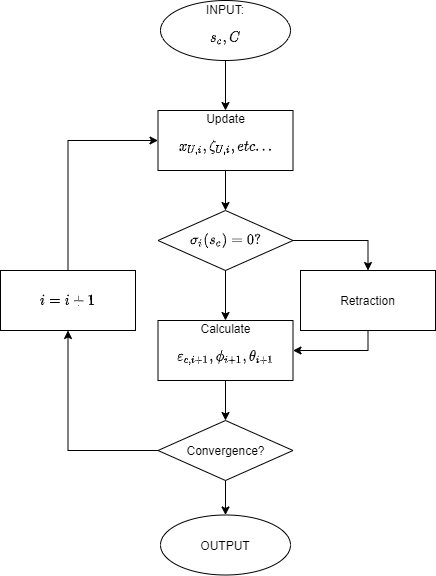
\includegraphics[width = 0.6\columnwidth]{figure/AmendFlow.png}
		%	\caption{A flow chart}
	%	\end{figure}
	
		はじめに,母線方向の曲線操作を行います.この際,$ \varepsilon $に関する要求は以下にまとめられます.
		\begin{itemize}
			\item $ s=0,L $で$ \varepsilon(s) = 0 $
			\item $ \varepsilon \geq 0 \forall s \in [0,L]$
			\item $ \varepsilon'>0 \forall s \in [ 0,s_c ) $
			\item $ \varepsilon'<0 \forall s \in ( s_c ,L] $
			\item $ \varepsilon(s_c) = \varepsilon_p $(極大値制約)
		\end{itemize}
		3番目と4番目の式を自動的に解消するため,$ \varepsilon' $を以下のように基底関数の線形和によって表す.
		\begin{equation}\label{eq:ver_Sdot_eq}
			\varepsilon' = \sum_{i=1}^N a_i s^i (s_c -s)
		\end{equation}
	 	なお,基底関数には多項式を用いている.$ \sum a_i s^i  >0\forall s \in [0,L]$が常に$ 0 $より大きければ,3番目と4番目の式を自動的に満たされるようになる.この文脈が常に成り立つ仮定で,局所的な変形が達成されるならば,以下の条件を満たす$ \bd{a} $を求める最適化問題になる.
	 	\begin{equation}\label{eq:var_st_min}
				\min_{\bd{a}} \int_{0}^L \varepsilon ds
	 	\end{equation}
		この問題の目的・制約条件は全て線形の形に書くことができるので,この最適化問題は線形計画問題の解法を用いることで解くことができる.
		
		しかし,この動作はあくまで母線方向のみ近づくことができるため,次の操作で恣意的に母線方向を変更させる.この時,局所修正を想定するときには下記の要求を満たす必要があります.
		\begin{itemize}
		\item $ \int |\sum_{j=1}^{n} \varepsilon_j \bd{d}_j|^2 ds  $が最小であること
 			\item $\min |\xv_{U,n}(s_c) + \varepsilon_{i+1} \bd{d}_{i+1} - \bd{C}| $
 		\end{itemize}
 		まずはじめに,$ \bd{d} = \bd{d}_1(s_c) \cos \psi + \bd{\eta}(s_c) \sin \psi $と表す.$ \bd{d}_1(s_c),  \bd{\eta}(s_c) $は$ s=s_c $の時の方向を参照しているだけであり,分布ではないことに注意する.この時,上記で述べた2つの条件は次式のように表される.
 		\begin{equation}\label{eq:No1_eq}
 			\varepsilon_{c,i+1}^2 \int_{0}^{L} \exp \left[ \int_{s_c}^{s} 2\sigma_{i+1} (s) \right] + 2\varepsilon_{c,i+1} \bd{d}_{i+1} \cdot \left[\int_{0}^{L} \sum_{j=1}^{i} \varepsilon_j \bd{d}_j \exp \left[ \int_{s_c}^{s} 2\sigma_{i+1} (s) \right] \right] + \int_{0}^{L} |\sum_{j=1}^{i} \varepsilon_j \bd{d}_j|^2 ds
 		\end{equation}
 		
 		\begin{equation}\label{eq:No2_eq}
 			\varepsilon_{c}^2 -2 \varepsilon_{c} \bd{d}\cdot (\bd{C}-\xv_{U,n}) + |\bd{C}-\xv_{U,n}|^2
 		\end{equation}
 	   式(\ref{eq:No2_eq})より,
 	   \begin{equation}\label{eq:var_eq_with_psi}
 	   		\varepsilon_{c} = \bd{d}_1 \cdot (\bd{C} - \xv_{U,n}) \cos \psi + \etav \cdot (\bd{C}-\xv_{U,n}) \sin \psi
 	   \end{equation}
    	これを式(\ref{eq:No1_eq})に代入し整理することで,$ \psi $の式として表すことができ,最小値を求めることができる.
    	
    \section{結果}
    この数値実験では,2つの円弧の間に形成された曲面を$ s=0.2 $の時の点を,$\bd{C} = [ 0.241197 0.308751 0.480096 ]$に変更したい場合を想定した結果となる.
    	\begin{figure}[H]
    		\begin{minipage}{0.5\hsize}
    			\centering
    			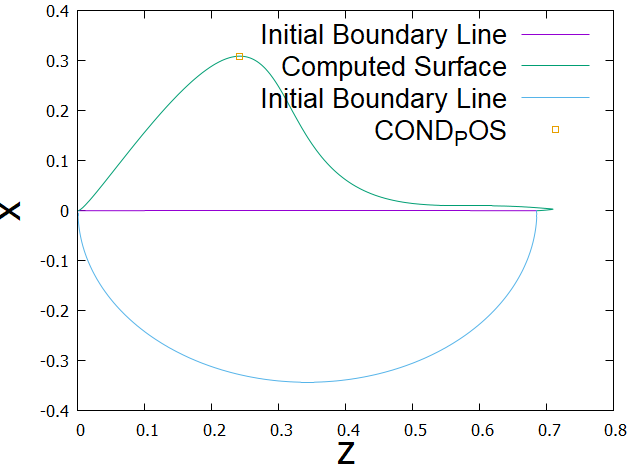
\includegraphics[width = 1.0\columnwidth]{figure/0409/ObtainedRidgeLinefromz-x.png}
    			\caption{z-x plane }
    		\end{minipage}
	    	\begin{minipage}{0.5\hsize}
	    		\centering
	    		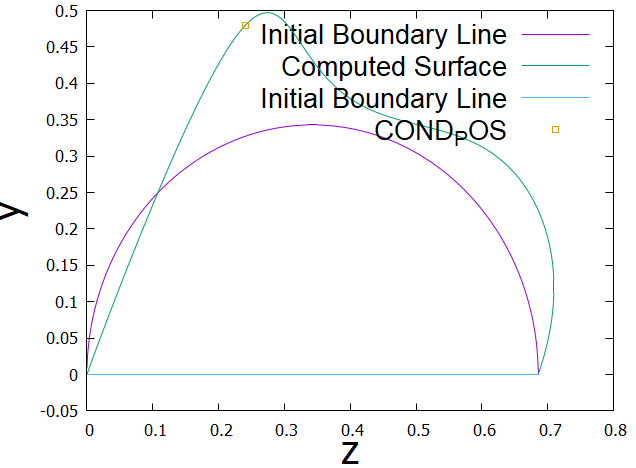
\includegraphics[width = 1.0\columnwidth]{figure/0409/ObtainedRidgeLinefromz-y.png}
	    		\caption{z-y plane }
	    	\end{minipage}
    	\end{figure}
   	\begin{figure}[H]
    		\centering
    		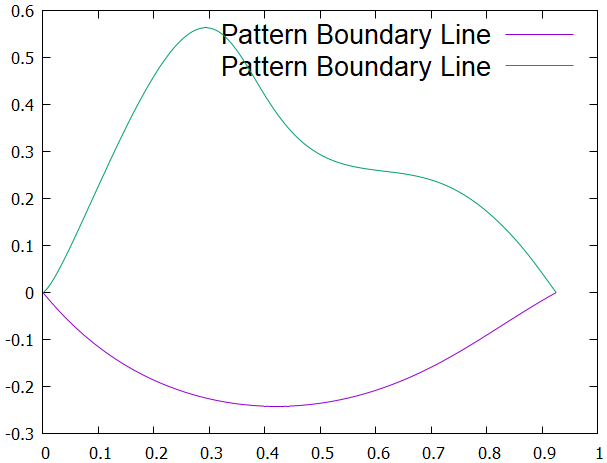
\includegraphics[width = 0.4\columnwidth]{figure/0409/Patt2.png}
    		\caption{z-y plane }
    \end{figure}
	この結果より,非常に曲線および曲面を局所的に変更することができたことが読み取れる.
		
	\section{次回のMTGについて(終了後記載)}
	\begin{itemize}
		\item  
		\item 
	\end{itemize}
	###
	\newpage
%\vspace{10cm}
%%%%%%%%%%%%%%%%%%%%%%%%%%%%%%%%%%%%%%
% 3.達成できなかったこととその問題点
	%\articleSPRthree
	
%%%%%%%%%%%%%%%%%%%%%%%%%%%%%%%%%%%%%%

%\vspace{14cm}
%%%%%%%%%%%%%%%%%%%%%%%%%%%%%%%%%%%%%%
	%\articleSPRfour
	%\articleSPRfive
\end{document}
